\newpage

\section{Введение}

\vspace{0.5cm}
\hspace{0.6cm}
В рамках производстенной практики необходимо было реализовать базу данных на MS SQL со связкой с C Sharp. 

\section{Сфера деятельности компании}

\vspace{0.5cm}
\hspace{0.6cm}
Компания «Цезарь Сателлит» - ведущий оператор систем безопасности для автомобилей и недвижимости.

\vspace{0.1cm}
Группа компаний «Цезарь Сателлит», созданная в 2000 году, является основателем и ключевым поставщиком рынка телематических услуг и комплексной безопасности на территории России. Более 200 000 частных клиентов и собственников бизнеса доверили компании самое дорогое: личную безопасность, защиту автомобиля, дома и офиса.

\vspace{0.1cm}
Использование новейших спутниковых (ГЛОНАСС/GPS) и мобильных (GSM) технологий, собственные патентованные разработки, развитая мониторинговая инфраструктура, уникальные технологии розыска и тесное взаимодействие с полицией – все это позволяет компании идти на опережение и противостоять современным методам угона.

\vspace{0.1cm}
Клиентами компании являются лидеры автомобильной промышленности, такие как BMW Russland Trading, Toyota Motor, Jaguar Land Rover, Mazda Motor Rus, Ford Sollers и крупнейшие автодилеры по всей стране. Под охраной «Цезарь Сателлит» находится значительная доля банковского сектора (Сбербанк, Райффайзенбанк, Ситибанк, Абсолют банк, Росбанк, БинБанк), ключевые сети розничной торговли (X5 Retail Group, «Азбука вкуса», «Магнит», «Дикси»).

\vspace{0.1cm}
Ежедневно «Цезарь Сателлит» предотвращает десятки случаев краж и автомобильных угонов по всей территории России, в странах Европы, Азии и СНГ, обеспечивая сохранность жизни и имущества своих клиентов\cite{csat}.


\newpage
\section{Основная часть}

\vspace{0.5cm}
\hspace{0.6cm}
Для реализации поставленной задачи была выбрана система управления реляционными базами данных, разработанная копорацие Microsoft, Microsoft SQL Server 2017. Выбор MS SQL 2017 был обусловлен стабильностью работы и совместимостью с языком программирования C Sharp. База данных, написанная на MS SQL, может подключится к C Sharp по прямому подключению, а также по подключению через   фреймворк Entity.



\subsection{Python}

\vspace{0.5cm}
\hspace{0.6cm}
Язык программирования Python использовался для генерации случайных данных для базы данных. Так как заполнение базы данных и придумывание осмысленных данных для ее атрибутов слишком трудозатратная задача, поэтому была выбрана библиотека генерации случайных данных - Faker. С ее помощью было сгенерировано более десяти тысяч строк данных, сравнимых с данными.

\vspace{0.1cm}
Faker - это библиотека Python, которая генерирует поддельные данные. Независимо от того, нужно ли нам загрузить свою базу данных, создать красивые XML-документы, заполнить наш тестотовый сервис, чтобы протестировать его, или анонимизировать данные, взятые из производственной службы.

\begin{lstlisting}[caption=Создание фейковых имен, label = list:pythonFakerName]
	from faker import Faker
	
	fake = Faker()
	
	for _ in range(3):
		print(fake.name())
	
	# 'Elda Palumbo'
	# 'Sig. Alighieri Monti'
	# 'Costanzo Costa'

\end{lstlisting}

\begin{lstlisting}[caption=Генерация фейковых адресов, label = list:pythonFakerAddresses]
	from faker import Faker

	fake = Faker()

	for _ in range(3):
		print(fake.address())

	# Michael Pike Dannyton, AR 20235
	#  Little Wall Apt. 359 East Loretta, NV 16913
	# Steve Park East Austin, MI 06826

\end{lstlisting}

\begin{lstlisting}[caption=Скрипт для генерации контрактов, label = list:GenerateContractsPy]
	from faker import Faker
	import random
	
	myFaker = Faker('en_US')

	f = open('/Users/antontimonin/Desktop/Practice/data/Contract1.txt', 'w')

	diaposon = 1001

	card_ids = []
	person_ids = []
	service_ids = []

	def formateDate(year):
		if year >= 0 and year < 10:
			return "0" + str(year)
		else:
			return str(year)

	for i in range(diaposon):
		f.write(str(i+1) + ';') #contract id
		while (1): 
			number = myFaker.pyint(min_value=1, max_value=350, step=1)
			if (number not in card_ids or len(card_ids) >= 350):
				card_ids.append(number)
				f.write(str(number) + ';') #car id
				break

		while (1): 
			number = myFaker.pyint(min_value=1, max_value=250, step=1)
			if (number not in person_ids or len(person_ids) >= 250):
				person_ids.append(number)
				f.write(str(number) + ';') #person id
				break

		while (1): 
			number = myFaker.pyint(min_value=1, max_value=15, step=1)
			if (number not in service_ids or len(service_ids) >= 15):
				service_ids.append(number)
				f.write(str(number) + ';') #service id
				break  

		day1 = myFaker.pyint(min_value=1, max_value=28, step=1)
		month1 = myFaker.pyint(min_value=1, max_value=12, step=1)
		year1 = myFaker.pyint(min_value=0, max_value=20, step=1)

		day2 = myFaker.pyint(min_value=1, max_value=28, step=1)
		month2 = myFaker.pyint(min_value=1, max_value=12, step=1)
		year2 = myFaker.pyint(min_value=0, max_value=20, step=1)

		if year1 < year2:
			day1, day2 = day2, day1
			month1, month2 = month2, month1
			year1, year2 = year2, year1
		elif year1 == year2 :
			if month1 < month2:
				day1, day2 = day2, day1
				month1, month2 = month2, month1
				year1, year2 = year2, year1
			elif month1 == month2:
				if day1 <= day2:
					day1, day2 = day2, day1
					month1, month2 = month2, month1
					year1, year2 = year2, year1

		date2 = str(day1) + "." + formateDate(month1) + "." + formateDate(year1)
		date1 = str(day2) + "." + formateDate(month2) + "." + formateDate(year2)

		f.write(date1 + ';') #date start id
		f.write(date2) #date end id
		f.write('\n')

	f.close()

\end{lstlisting}


\newpage
\subsection{MS SQL}

\vspace{0.5cm}
\hspace{0.6cm}
На языке SQL было создано две базы данных, предназначенных для оперативного взаимодействия всех компонентов компании. Главной таблицой в базе данных CS1 является таблица Contract. Эта таблица связывает все таблицы в двух базах данных. Через эту таблицу можно получить информацию о машинах оперделенного пользователя, какие сообщение приходили на оборудование, устоновленные в этой машине. Также можно определить в каком сервисном центре клиент устанавливал оборудование и когда это оборудование последний раз проверялось.

\vspace{0.1cm}
База данных, представленная на рисунке \ref{img:db_cs} спроектирована и приведена третьей нормальной форме.

\newpage
\begin{figure}[H]
	\centering
	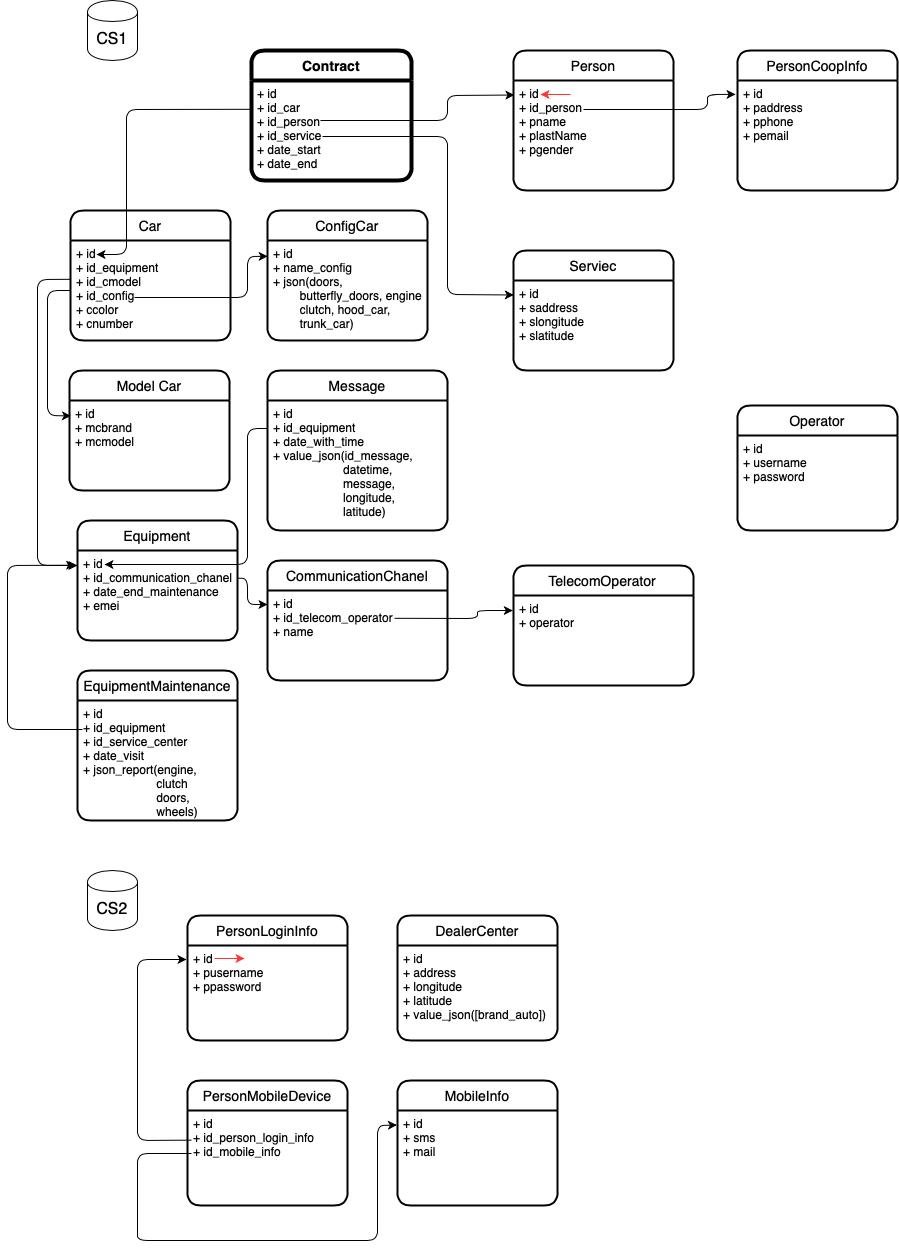
\includegraphics[scale=0.52]{img/bd_cs.png}
	\caption{Спроектированная база данных}
	\label{img:db_cs}
\end{figure}


\newpage
\vspace{0.5cm}
База данных CS1 состоит из следующих таблиц:
\begin{itemize}
	\item \textbf{Contract}- таблица с контрактами пользователей;
	\item \textbf{Person} - таблица с именем и фамилией клиента;
	\item \textbf{PersonCoopInfo} - таблица с контактами, по которым можно связать с клиентами;
	\item \textbf{Serviec} - таблица с адресами сервисов, устанавливающих оборудование компании клиентам;
	\item \textbf{Operator} - таблица с логинами и паролями операторов, мониторящих события, происходящие с имуществом клиентов;
	\item \textbf{Car} - таблица с номером и цветом машины клиента;
	\item \textbf{ConfigCar} - таблица с конфигурацией оборудования, поставленного на конкретную машину;
	\item \textbf{ModelCar} - таблица с брендом и моделью машины клиента;
	\item \textbf{Equipment} -  таблица с информаций об оборудование;
	\item \textbf{EquipmentMaintenance} - таблица с информацией о последнем техническом осмотре оборудования;
	\item \textbf{Message} - таблица с сообщениями, пришедшими на конкретное оборудование;
	\item \textbf{CommunicationChanel} - таблица с каналом коммуникации, установленным в оборудование;
	\item \textbf{TelecomOperator} - таблица с операторами связи.
	
\end{itemize}

\vspace{0.5cm}
База данных CS2 состоит из следующих таблиц:
\begin{itemize}
	\item \textbf{PersonLoginInfo}- таблица с логинами и паролями пользователей, для входа в систему для мониторинга состояния их имущества;
	\item \textbf{PersonMobileDevice}- таблица информацией о включенных функциях на мобильных устройствах;
	\item \textbf{MobileInfo}- таблица с информацией о включенных методах оповещения;
	\item \textbf{DealerCenter}- таблица с информацией о местоположении дилерских центров.
\end{itemize}

На листингах \ref{list:GetConcreteCarByID}-\ref{list:AddNewCommunicationChanel} приведены запросы к базам данных CS1 и CS2.

\begin{lstlisting}[caption=Функция поиска информации по автомобилям по пользовательскому id, label = list:GetConcreteCarByID]
	CREATE FUNCTION GetConcreteCarByID (@id_person int)  
	RETURNS TABLE  
	AS  
	RETURN   
	(  
		SELECT c.id, p.pname, p.plastname, pinf.paddress, pinf.pemail, pinf.pphone, mc.mcbrand, mc.mcmodel, cr.cnumber 
		FROM Contracts as c
		JOIN Person AS p ON p.id = c.id_person
		JOIN PersonInfo AS pinf ON pinf.id = p.id_personinfo
		JOIN Car AS cr ON cr.id = c.id_car
		JOIN ModelCar as mc ON mc.id = cr.id_cmodel
		WHERE c.id = @id_person
	);

	SELECT * FROM GetConcreteCarByID(15);

	DROP FUNCTION GetConcreteCarByID;
\end{lstlisting}

\begin{lstlisting}[caption=Хранимая процедура\,выводящая полную информацию по id контракта, 
label = list:AddAllInfo]
	CREATE PROCEDURE AddAllInfo(@id_contract int) AS
	BEGIN
		DROP TABLE IF EXISTS dbo.TmpFullInfo

	create TABLE CS.dbo.TmpFullInfo(
		id int NOT NULL,
		person_name VARCHAR(100) NOT NULL,
		person_lastname VARCHAR(100) NOT NULL,
		person_address VARCHAR(100) NOT NULL,
		person_email VARCHAR(100) NOT NULL,
		person_phone VARCHAR(100) NOT NULL,
		service_address VARCHAR(100) NOT NULL,
		car_brand VARCHAR(100) NOT NULL,
		car_model VARCHAR(100) NOT NULL,
		car_number VARCHAR(100) NOT NULL
	)

		insert into dbo.TmpFullInfo
		SELECT c.id, p.pname, p.plastname, pinf.paddress, pinf.pemail, 
					 pinf.pphone, s.saddress, mc.mcbrand, mc.mcmodel, cr.cnumber FROM Contracts as c
		JOIN Serviec AS s ON s.id = c.id_service
		JOIN Person AS p ON p.id = c.id_person
		JOIN PersonInfo as pinf ON pinf.id = p.id_personinfo
		JOIN Car AS cr ON cr.id = c.id_car
		JOIN ModelCar as mc ON mc.id = cr.id_cmodel
		WHERE c.id = @id_contract
	END;

	exec AddAllInfo 3;

	select * from TmpFullInfo;

	drop procedure AddAllInfo;

	select * from TmpFullInfo;
\end{lstlisting}

\begin{lstlisting}[caption=Функция для вывода полной информации по пользователям, label = list:GetFullInfoAboutPerson]
	DROP FUNCTION GetFullInfoAboutPerson;

	CREATE FUNCTION GetFullInfoAboutPerson()  
	RETURNS TABLE  
	AS  
	RETURN   
	(  
		SELECT p.id, p.pname, p.plastname, pinf.pemail, plog.pusername, plog.ppassword FROM CS.dbo.Person as p
		JOIN CS.dbo.PersonInfo as pinf ON pinf.id = p.id_personinfo
		JOIN CS2.dbo.PersonLoginInfo AS plog ON plog.id = p.id
	);

	SELECT * FROM GetFullInfoAboutPerson();
\end{lstlisting}

\begin{lstlisting}[caption=Процедура для формирования нового контракта с проставлением всех зависимостей, label = list:FormContract]
	CREATE PROCEDURE FormContract(@person_name VARCHAR(100), 
															 @person_lastname VARCHAR(100),
														 	@person_gender VARCHAR(100),
															 @person_phone VARCHAR(100),
															 @car_brand VARCHAR(100),
															 @car_model VARCHAR(100),
															 @car_color VARCHAR(100),
															 @car_number VARCHAR(100),
															 @equipment_emei VARCHAR(100),
															 @operator VARCHAR(100)) AS
	DECLARE 
		-- Contract
		@ID_CONTRACT INT,
		@DATE_START DATE,
		@DATE_END DATE,

		-- Person
		@ID_PERSON INT,
		@ID_PERSON_COOP_INFO INT,

		-- Car
		@ID_CAR INT,
		@ID_EQUIPMENT INT,
		@ID_MODELCAR INT,
		@ID_CONFIG INT,

		-- Communication Chanel
		@ID_COMMUNICATION_CHANEL INT

	BEGIN

		SELECT @DATE_START = CONVERT(DATE, GETDATE());
		SELECT @DATE_END = CONVERT(DATE, DATEADD(year, 8, GETDATE()));

		SELECT @ID_COMMUNICATION_CHANEL = 1;
		SELECT @ID_CONFIG = 1;

		SELECT @ID_MODELCAR = mc.id FROM CS.dbo.ModelCar as mc
		WHERE mc.mcbrand = @car_brand and mc.mcmodel = @car_model

		IF NOT EXISTS (SELECT mc.id FROM CS.dbo.ModelCar as mc WHERE mc.id = @ID_MODELCAR)
		BEGIN
			INSERT INTO CS.dbo.ModelCar(mcbrand, mcmodel)
			VALUES (@car_brand, @car_model);
			SET @ID_MODELCAR = (SELECT SCOPE_IDENTITY());
		END;

		EXEC GetConfigID @car_brand;
		SELECT @ID_CONFIG = tt.num_id_operator FROM CS.dbo.TmpTable as tt;

		-- Add in Equipment table
		INSERT INTO CS.dbo.Equipment(id_communication_chanel, date_end_maintenance, emei)
		VALUES (@ID_COMMUNICATION_CHANEL, @DATE_END, @equipment_emei);
		SET @ID_EQUIPMENT = (SELECT SCOPE_IDENTITY());

		-- Add in Car table
		INSERT INTO CS.dbo.Car(id_equipment, id_cmodel, id_config, ccolor, cnumber)
		VALUES (@ID_EQUIPMENT, @ID_MODELCAR, @ID_CONFIG, @car_color, @car_number);
		SET @ID_CAR = (SELECT SCOPE_IDENTITY());

		-- Add in PersonInfo table
		INSERT INTO CS.dbo.PersonInfo(paddress, pphone, pemail)
		VALUES ('', @person_phone, '');
		SET @ID_PERSON_COOP_INFO = (SELECT SCOPE_IDENTITY());

		-- Add in Person table
		INSERT INTO CS.dbo.Person(id_personinfo, pname, plastname, pgender)
		VALUES (@ID_PERSON_COOP_INFO, @person_name, @person_lastname, @person_gender);
		SET @ID_PERSON = (SELECT SCOPE_IDENTITY());

		-- Add in Contracts table
		INSERT INTO CS.dbo.Contracts(id_car, id_person, id_service, date_start, date_end)
		VALUES (@ID_CAR, @ID_PERSON, 0, @DATE_START, @DATE_END);
		SET @ID_CONTRACT = (SELECT SCOPE_IDENTITY());
		END;

	exec FormContract 'Bar', 'Baz', 'Man', 'email@mail.ru', 'BMW', 'X1', 'Bluebi', 'TT777T777', 	'JKWNNGKWEJNGKWE', 'Yota';
	
	drop procedure FormContract;

\end{lstlisting}

\begin{lstlisting}[caption=Процедура для удаления контрака\, с удалением всех необходимых зависимостей для вывода полной информации по пользователям, label = list:DeleteContractWithID]
	CREATE PROCEDURE DeleteContractWithID(@ID INT) AS
	DECLARE 
		@ID_PERSON INT,
		@ID_PERSON_COOP_INFO INT,
		@ID_CAR INT,
		@ID_EQUIPMENT INT;
	BEGIN

		SELECT @ID_PERSON = c.id_person FROM CS.dbo.Contracts as c
		WHERE c.id = @ID;

		SELECT @ID_PERSON_COOP_INFO = p.id_personinfo FROM CS.dbo.Person as p
		WHERE p.id = @ID_PERSON;

		SELECT @ID_CAR = c.id_car FROM CS.dbo.Contracts as c
		WHERE c.id = @ID;

		SELECT @ID_EQUIPMENT = cr.id_equipment FROM CS.dbo.Car as cr
		WHERE cr.id = @ID_CAR;

		-- DELETE CONTRACT
		DELETE FROM CS.dbo.Contracts
		WHERE CS.dbo.Contracts.id = @ID;

		-- DELETE PERSON
		IF EXISTS (SELECT @ID_PERSON) DELETE FROM CS.dbo.Person
		WHERE CS.dbo.Person.id = @ID_PERSON;

		-- DELETE PERSON COOP INFO
		IF EXISTS (SELECT @ID_PERSON_COOP_INFO) DELETE FROM CS.dbo.PersonInfo
		WHERE CS.dbo.PersonInfo.id = @ID_PERSON_COOP_INFO;

		-- DELETE CAR
		IF EXISTS (SELECT @ID_CAR) DELETE FROM CS.dbo.Car
		WHERE CS.dbo.Car.id = @ID_CAR;

		-- DELETE EQUIPMENT
		IF EXISTS (SELECT @ID_EQUIPMENT) DELETE FROM CS.dbo.Equipment
		WHERE CS.dbo.Equipment.id = @ID_EQUIPMENT;

		-- DELETE MESSAGES
		IF EXISTS (SELECT @ID_EQUIPMENT) DELETE FROM CS.dbo.Message
		WHERE CS.dbo.Message.id_equipment = @ID_EQUIPMENT;

		SELECT @ID, @ID_PERSON, @ID_PERSON_COOP_INFO, @ID_CAR, @ID_EQUIPMENT;
--delete message with id_equipment id
	END;

	drop procedure DeleteContractWithID;

	EXEC DeleteContractWithID 247;
\end{lstlisting}

\begin{lstlisting}[caption=Процедура для добавления нового канала коммуникации, label = list:AddNewCommunicationChanel]
	CREATE PROCEDURE AddNewCommunicationChanel(@name_communication VARCHAR(200)) AS
	DECLARE 
		@ID_COMMUNICATION_CHANEL INT,
		@ID_OPERATOR INT,
		@NAME_OPERATOR VARCHAR(200);
	BEGIN

		SELECT @NAME_OPERATOR = 
		CASE 
			WHEN @name_communication = 'MTC' THEN 'mtc_tech'
			WHEN @name_communication = 'Megafon' THEN 'megafon_tech'
			WHEN @name_communication = 'Tele2' THEN 'tele2_tech'
			WHEN @name_communication = 'Bilain' THEN 'bilain_tech'
			WHEN @name_communication = 'Yota' THEN 'yota_tech'
			WHEN @name_communication = 'Tinkoff' THEN 'tinkoff_tech'
			WHEN @name_communication = 'Vineah' THEN 'vineah_tech'
			ELSE 'unknown_tech'
		END;

		SELECT @ID_OPERATOR = toper.id FROM CS.dbo.TelecomOperator as toper
		WHERE toper.operator = @NAME_OPERATOR;

		INSERT INTO CS.dbo.CommunicationChanel(id_telecom_operator, name)
		VALUES (@ID_OPERATOR, @name_communication);
		SET @ID_COMMUNICATION_CHANEL = (SELECT SCOPE_IDENTITY());

		IF (object_id('CS.dbo.TmpTable','U')) IS NOT NULL
		BEGIN
			DROP TABLE CS.dbo.TmpTable;
		END;

		CREATE TABLE CS.dbo.TmpTable(
			num_id_operator int NOT NULL
		);

		INSERT INTO CS.dbo.TmpTable (num_id_operator)
		VALUES (@ID_COMMUNICATION_CHANEL);
	END;

	EXEC AddNewCommunicationChanel 'Yota';
	
	drop procedure AddNewCommunicationChanel;

\end{lstlisting}


\subsection{C Sharp}

\vspace{0.5cm}
\hspace{0.6cm}
С Sharp (произносится как "си шарп") — современный объектно-ориентированный и типобезопасный язык программирования. C Sharp относится к широко известному семейству языков C, и покажется хорошо знакомым любому, кто работал с C, C++, Java или JavaScript.

\vspace{0.1cm}
C Sharp является объектно-ориентированным языком, но поддерживает также и компонентно-ориентированное программирование. Разработка современных приложений все больше тяготеет к созданию программных компонентов в форме автономных и самоописательных пакетов, реализующих отдельные функциональные возможности. Главная особенность таких компонентов в том, что они представляют собой модель программирования со свойствами, методами и событиями. У них есть атрибуты, предоставляющие декларативные сведения о компоненте. Они включают в себя собственную документацию. C Sharp предоставляет языковые конструкции, непосредственно поддерживающие такую концепцию работы. Благодаря этому C Sharp подходит для создания и применения программных компонентов\cite{microsoft-csharp}.

\vspace{0.1cm}
На листинге \ref{list:csDataBase} представлен класс, отвечающий за подключение к базе данных MS SQL Server.

\begin{lstlisting}[caption=Подключение к базе данных, label = list:csDataBase]
	class CS_DB
	{
		private SqlConnection connection = new SqlConnection("Data Source=4D97\\MSSSQLSERVER;Initial Catalog=CS;Integrated Security=True");
	
		public void openConnection()
		{
			if (connection.State == ConnectionState.Closed)
			{
				connection.Open();
			}    
		}
	
		public void closeConnection()
		{
			if (connection.State == ConnectionState.Open)
			{
				connection.Close();
			}
		}
	
		public SqlConnection getConnection()
		{
			return connection;
		}
	}
\end{lstlisting}

\subsection{Windows Forms}

\vspace{0.5cm}
\hspace{0.6cm}
Windows Forms позволяет разрабатывать интеллектуальные клиенты. Интеллектуальный клиент — это приложение с полнофункциональным графическим интерфейсом, простое в развертывании и обновлении, способное работать при наличии или отсутствии подключения к Интернету и использующее более безопасный доступ к ресурсам на локальном компьютере по сравнению с традиционными приложениями Windows \cite{microsoft-wondowsforms}.

Пример создание формы через Windows Forms API представлен на листинге \ref{list:csCreateForm}. На рисунке \ref{img:auth}, \ref{img:main_1}, \ref{img:main_2} представлены форма авторизации оператора, главная форма с информацией о пользователе, форма с информацией о машинах конкретного пользователя соответственно. 

\begin{lstlisting}[caption=Пример создания формы в программе оператора, label = list:csCreateForm]
	public partial class FormAuth : Form
	{
		ControllerFormAuth controller;
		public FormAuth()
		{
			InitializeComponent();
	
			this.controller = new ControllerFormAuth();
		}
	
		private void loginButton_Click(object sender, EventArgs e)
		{
	
			if (controller.IsLogged(usernameTextBox.Text, passwordTextBox.Text))
			{
				this.Hide();
				Form1 nextWindow = new Form1(usernameTextBox.Text, passwordTextBox.Text);
				nextWindow.ShowDialog();
			}
			else
			{
				MessageBox.Show("This operator does not exist");
			}
		}
	}
\end{lstlisting}

\begin{figure}[H]
	\centering
	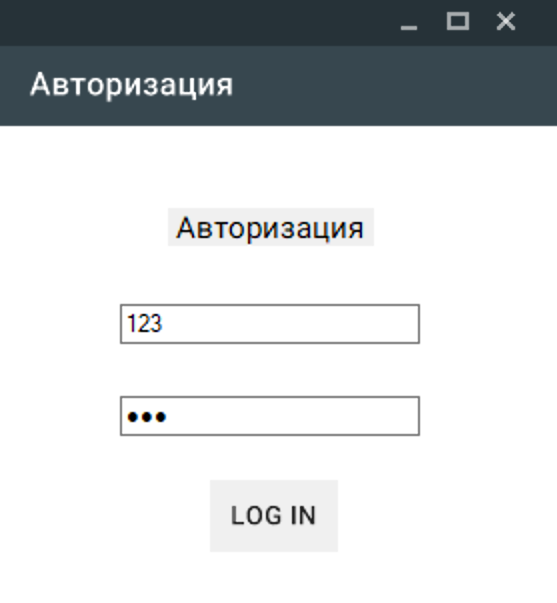
\includegraphics[scale=0.9]{img/auth.png}
	\caption{Форма авторизации}
	\label{img:auth}
\end{figure}

\begin{figure}[H]
	\centering
	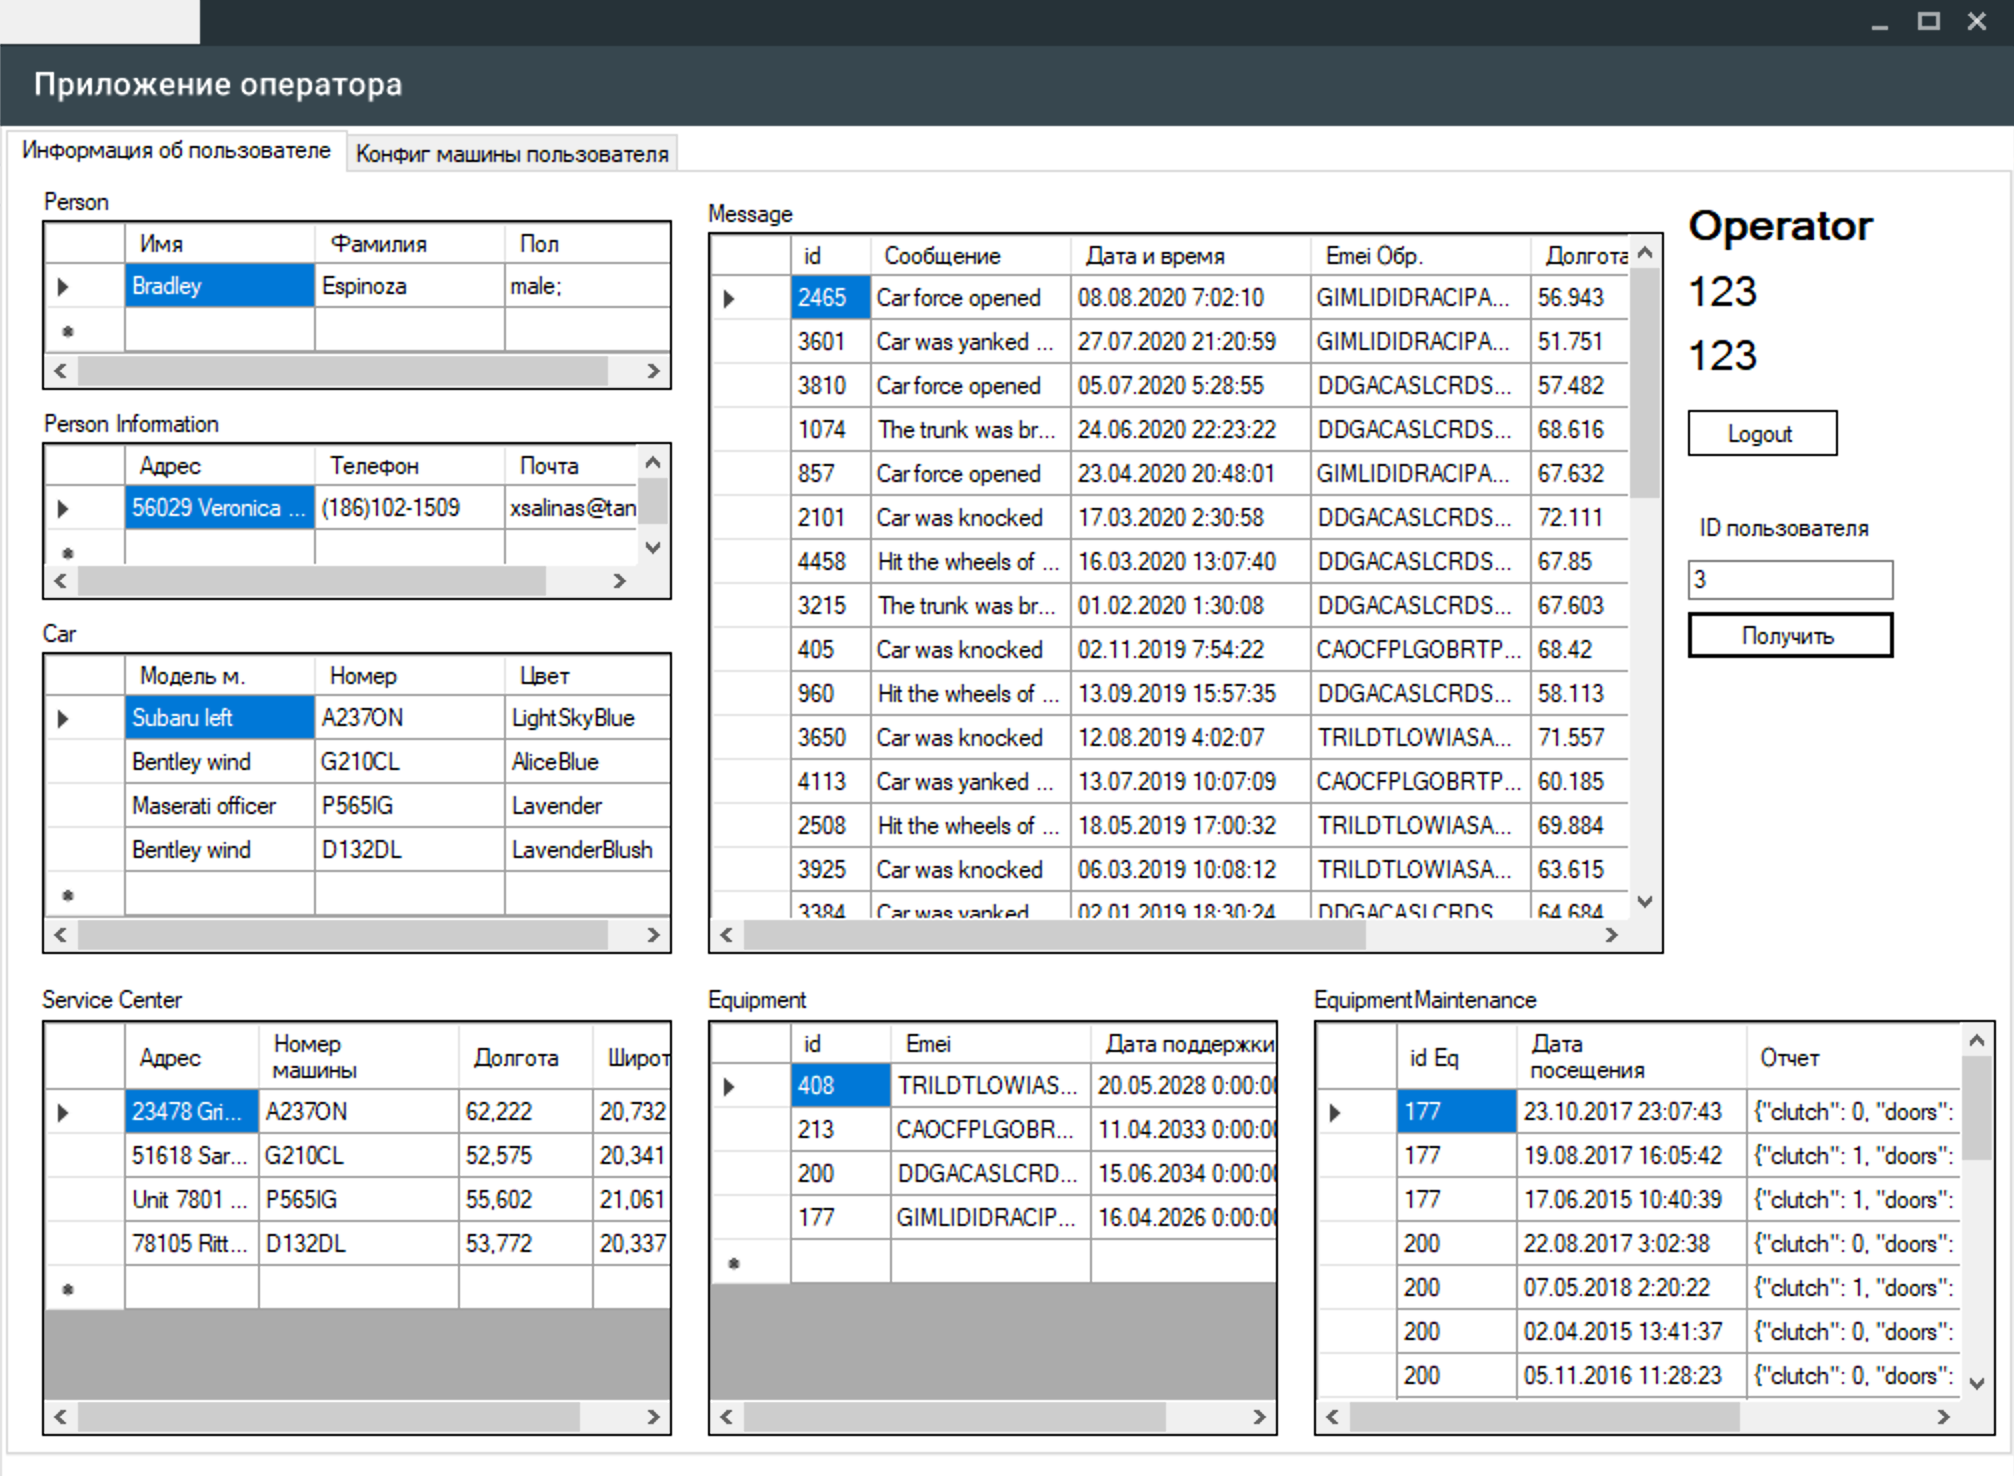
\includegraphics[scale=0.5]{img/main_1.png}
	\caption{Форма со всей информацие о пользователе}
	\label{img:main_1}
\end{figure}

\begin{figure}[H]
	\centering
	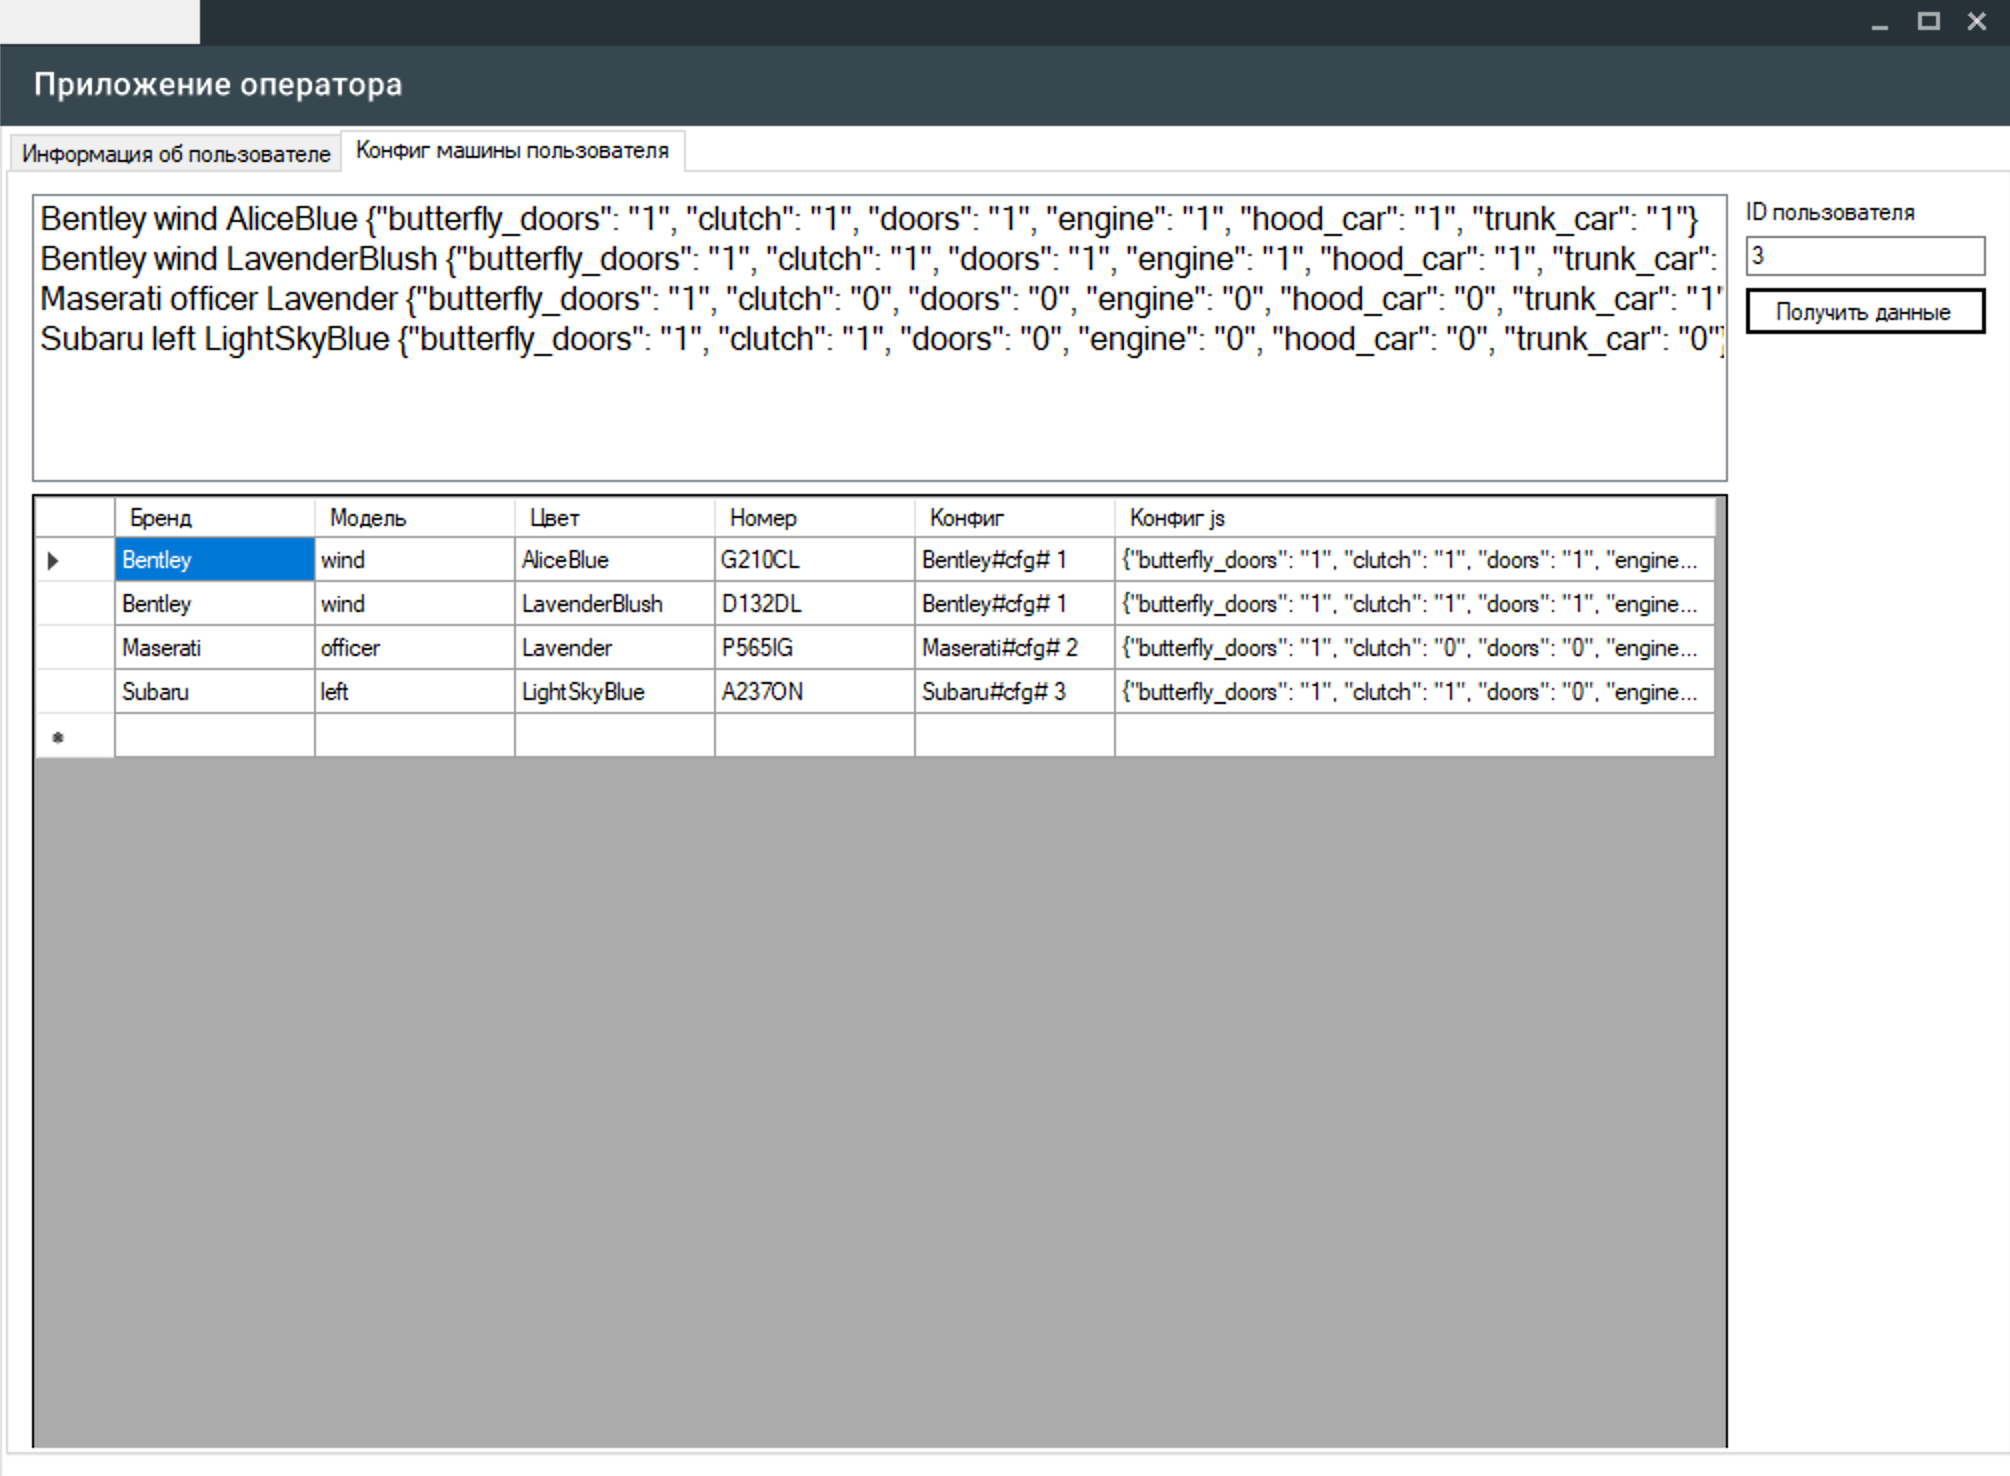
\includegraphics[scale=0.5]{img/main_2.png}
	\caption{Форма с информацией об машине пользователя}
	\label{img:main_2}
\end{figure}

\subsection{Entity Framework}
\vspace{0.5cm}
\hspace{0.6cm}
Entity Framework — это набор технологий в ADO.NET, которые поддерживают разработку программных приложений, ориентированных на данные. Архитекторам и разработчикам приложений, ориентированных на обработку данных, приходится учитывать необходимость достижения двух совершенно различных целей. Они должны моделировать сущности, связи и логику решаемых бизнес-задач, а также работать с ядрами СУБД, используемыми для сохранения и получения данных. Данные могут распределяться по нескольким системам хранения данных, в каждой из которых применяются свои протоколы, но даже в приложениях, работающих с одной системой хранения данных, необходимо поддерживать баланс между требованиями системы хранения данных и требованиями написания эффективного и удобного для обслуживания кода приложения.

Платформа Entity Framework позволяет работать с данными в форме специфических для домена объектов и свойств (например, с клиентами и их адресами) без необходимости учитывать формат базовых таблиц и столбцов базы данных, где хранятся эти данные. Entity Framework дает разработчикам возможность работать с данными на более высоком уровне абстракции, создавать и сопровождать приложения, ориентированные на работу с данными, одновременно с этим сокращая объем кода по сравнению с традиционными приложениями. Поскольку Entity Framework является компонентом .NET Framework, Entity Framework приложения могут работать на любом компьютере, на котором установлена .NET Framework с пакетом обновления 1 (SP1) версии 3,5. \cite{microsoft-entityframework}

На практике по фреймворку Entity  была дана теоретическа информация с последующим самостоятельным изучением.

\newpage
\section{Заключительная часть}

\vspace{0.5cm}
\hspace{0.6cm}
Разработана база данных в связке с десктопным приложением, позволяющим авторизироваться операторам мониторинга и посмотреть всю информацию о клиенте. За время практики база данных приложение для операторов связи было переведено с обычного подключения базы данных к серверу MS SQL на подключение через строку подключения и фреймворк Entity.
